\subsection{Pneumatics}

    Most industrial operations require objects to be moved from one location to another - this is achieved through mechanical movement driven by prime movers \cite{parr2011hydraulics}. Prime movers are the power houses of industrial operations. Electric motors are a common choice for prime movers as rotary and linear movement can be achieved through either and or a direct or geared coupling to the motor shaft\cite{parr2011hydraulics}. Electric motors are not the only option as movement can be facilitated through subsequent flow of fluid - liquid and gas\cite{parr2011hydraulics}. Hydraulics is the name given to liquid-based systems and Pneumatics is the name given to air-based systems. The nature of the application will dictate whether an electric, hydraulic, pneumatic or a combination of each should be implemented. For example - pneumatics are common within the food processing industry as a leak in the pneumatic line will not spoil the food. Figure \ref{fig:pnemumaticSystem} illustrates a simplified overview of the necessary components required for a pneumatic system. 
    All mechanical movement within the lolly machine is driven by pneumatic actuators. As the lolly machine is portable, the pneumatic system supplying the machine will vary depending on location.
    
    \begin{figure}[H]
        \centering
        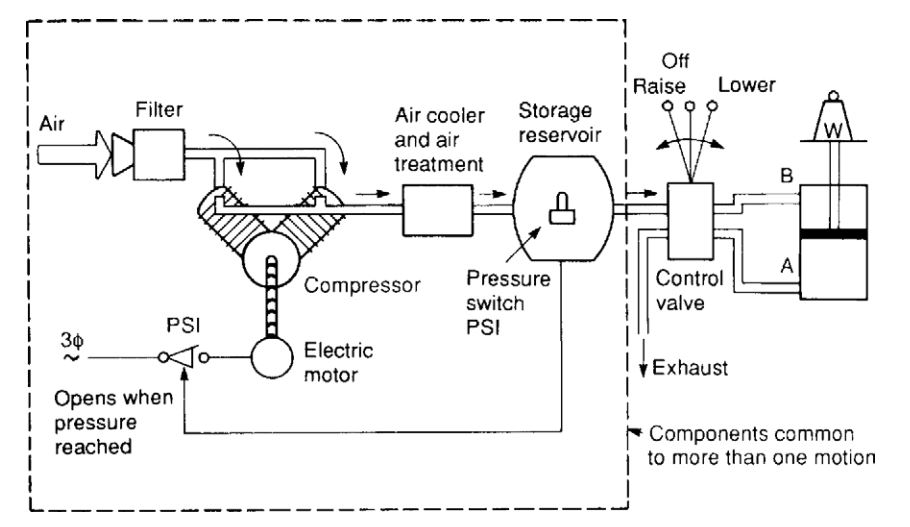
\includegraphics[scale = 0.6]{pneumaticSystem.JPG}
        \caption{A simplified overview of a pneumatic system~\cite{parr2011hydraulics}.}
        \label{fig:pnemumaticSystem}
    \end{figure}
    \newpage
    
\subsection{Linear Actuators}
    Linear actuators, as the name suggests, provides linear movement to push and/or pull objects within a given process. The linear actuators on the lolly machine are powered by pneumatics. The main components of a linear actuator are as follows:
    
    \begin{description} 
        \item\textbf{Rod:} connects the actuator to the outside environment.
        \item\textbf{Piston:} facilitates movement to the rod through applied pressure to either side.
        \item\textbf{Barrel:} houses the piston.
        \item\textbf{Extend Port:} when air enters, the rod will extend outwards.
        \item\textbf{Retract Port:} When air enters, the rod will retract inwards.
    \end{description}
    
    The fundamental concept is that the differential pressure between either side of the piston will cause it to move\cite{parr2011hydraulics}. The direction of movement is dependent on the flow of air through the extend and retract ports.
    
    \begin{figure}[H] 
        \centering
        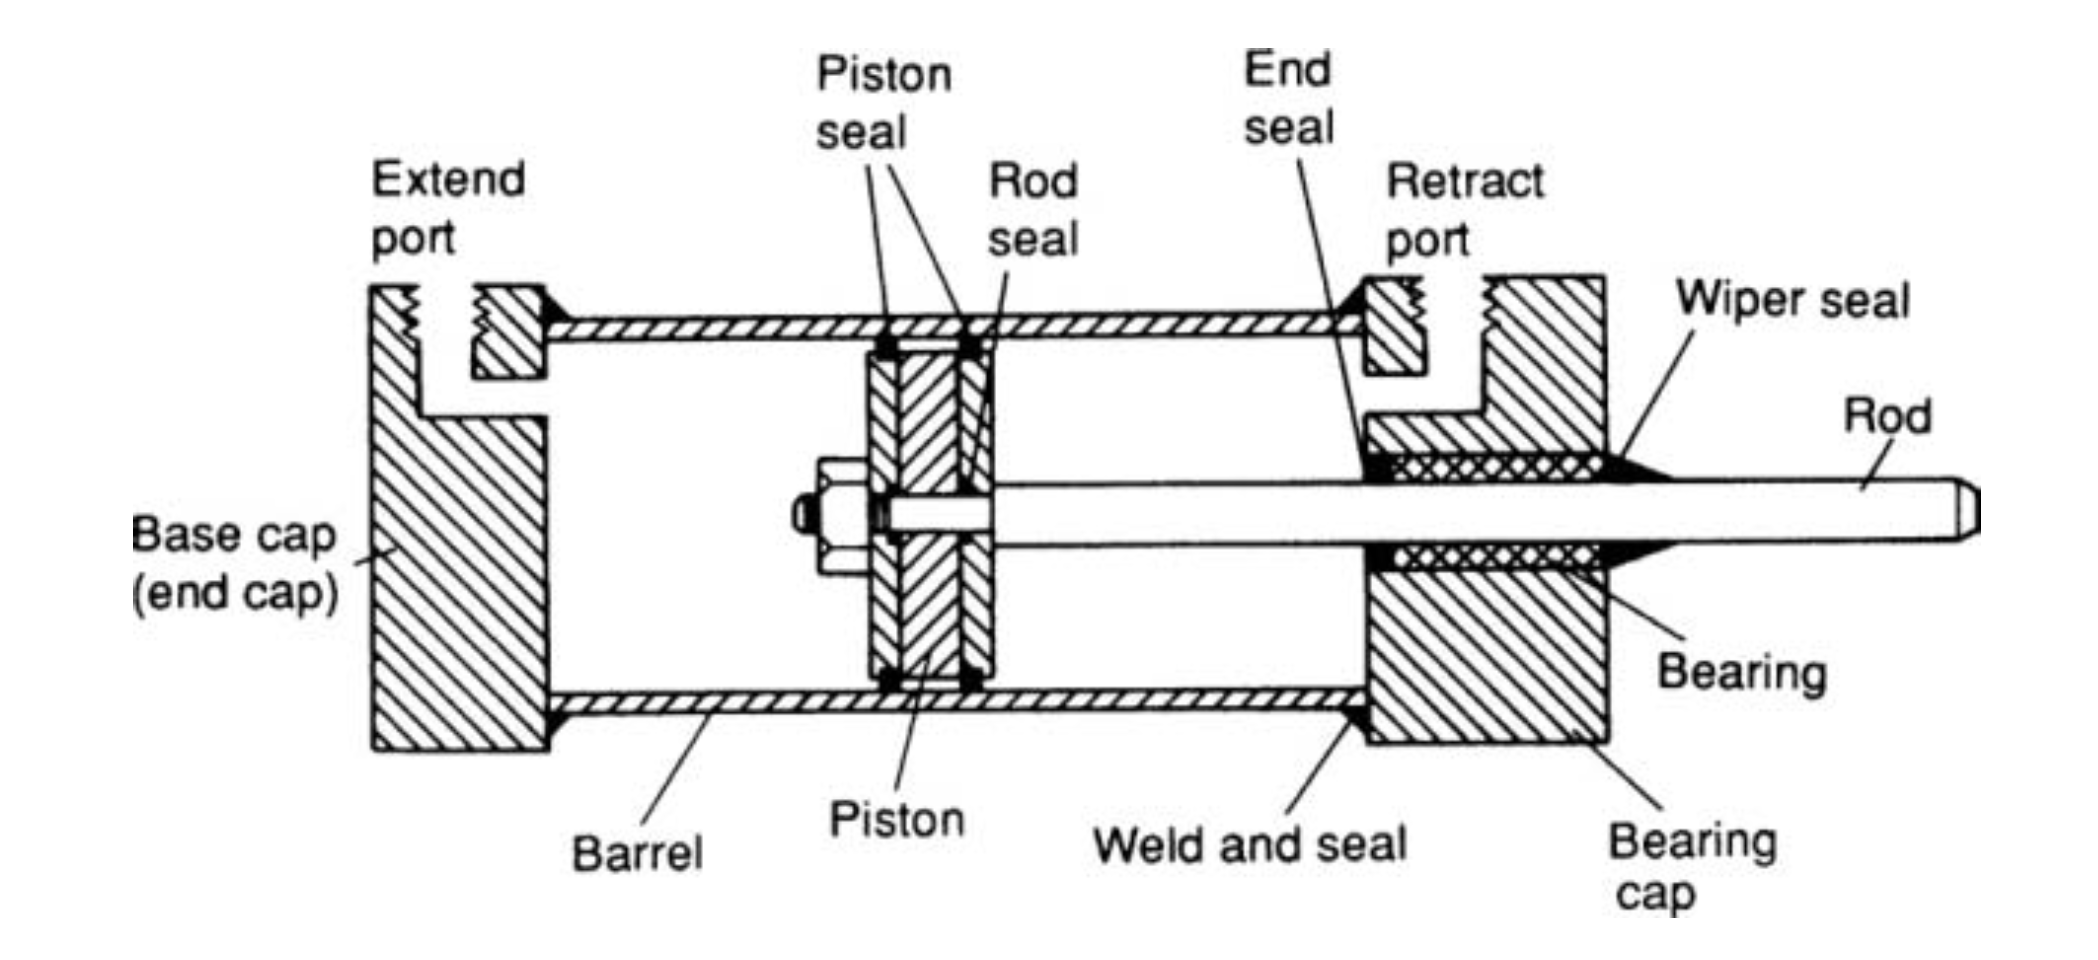
\includegraphics[width = 0.5\textwidth]{2_images/linearActuator.png}
        \caption{A cross section view of a linear actuator~\cite{parr2011hydraulics}.}
        \label{fig:linearActuator}
    \end{figure}
    
    There are eight linear actuators installed on the lolly machine. Three are used within the sorting process while five are required for dispensing. Figure \ref{fig:rejectAct} shows the linear actuator responsible for dropping lollies into the colour sensing shoot.

    \begin{figure}[H] 
        \centering
        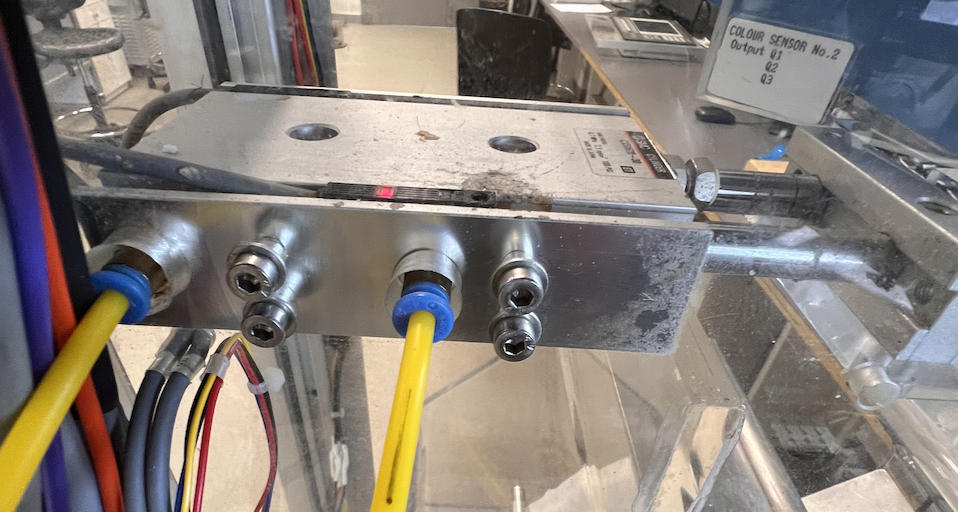
\includegraphics[width = 0.5\textwidth]{2_images/rejectAct.png}
        \caption{Lolly machine reject actuator.}
        \label{fig:rejectAct}
    \end{figure}        
\newpage     
\subsection{Rotary Actuators}
    Rotary actuators provide rotational movement to objects through a central shaft\cite{parr2011hydraulics}. Rotation can be restricted or unrestricted. A rack and pinion or vanes facilitate the turning action within the actuator\cite{parr2011hydraulics}. Rotary actuators within the lolly machine are driven by a single vane and restricted to 90$^{\circ}$\cite{smcRot}. Figure \ref{fig:rotaryActuator} shows a cross section of the \acrshort{smc} rotary actuators installed on the lolly machine. There are three rotary actuators installed on the lolly machine.
    
    \begin{figure}[H] % pushed to end
        \centering
        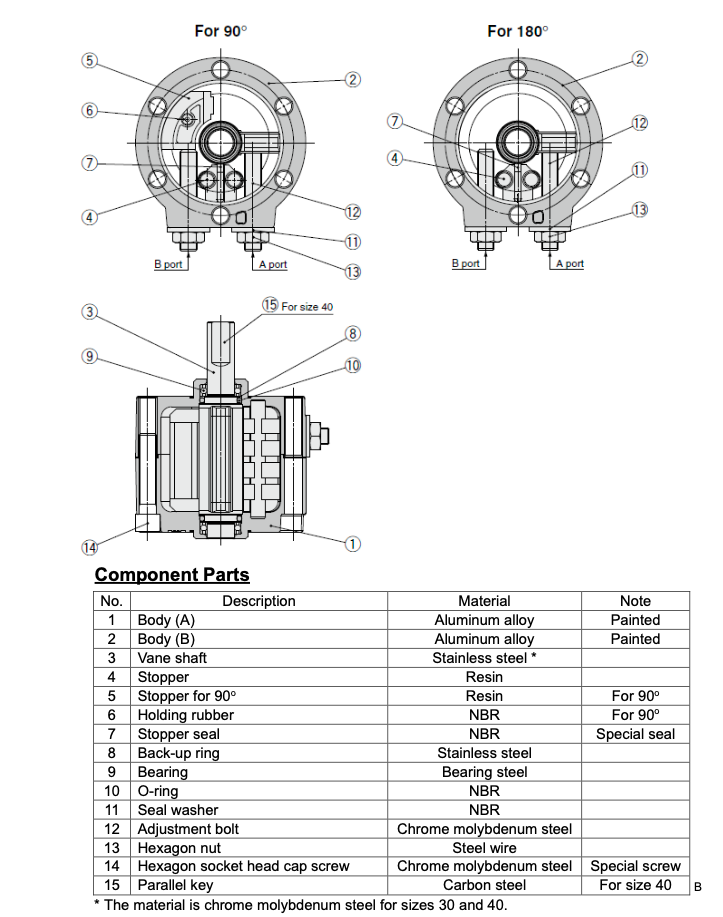
\includegraphics[scale = 0.4]{2_images/rotaryActuator.png}
        \caption{A cross section view of an \acrshort{smc} rotary actuator~\cite{smcRot}.}
        \label{fig:rotaryActuator}
    \end{figure}
\newpage
\subsection{Pneumatic Control Valves}
    Pneumatic control valves manage the air flow to pneumatic system peripherals. Control valves are defined by the number of ports, positions, and their control action\cite{parr2011hydraulics}. Figure \ref{fig:controlValves} compares two different types of valves - (a) shows a four-port two-position valve (4/2) while (b) shows a four-port, 3-position valve(4/2). Figure \ref{fig:controlValveConfig} shows a possible internal configuration for the 4/3 valve. It is important to note that the above mentioned figures do not represent typical pneumatic valve symbols and are included to illustrate the differences between various types of control valve configurations.
    
    \begin{figure}[H]
    \centering
    \begin{minipage}{0.45\textwidth}
        \centering
        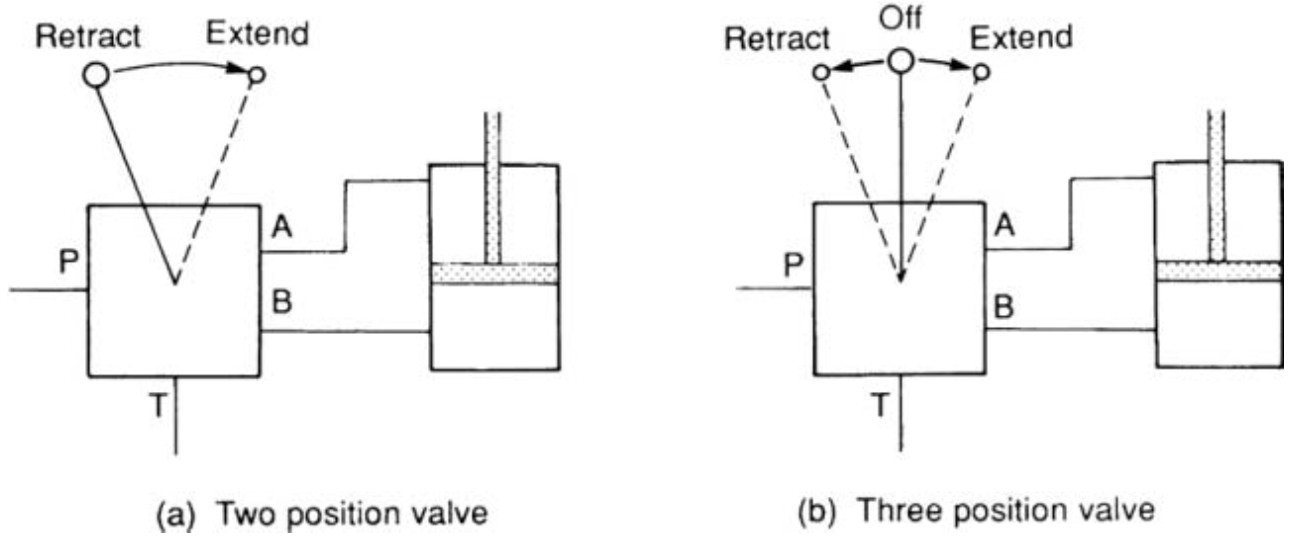
\includegraphics[width = 1\textwidth]{2_images/controlValves.png}
        \caption{Comparison between control valves~\cite{parr2011hydraulics}.}
        \label{fig:controlValves}
    \end{minipage}\hfill
    \begin{minipage}{0.5\textwidth}
        \centering
        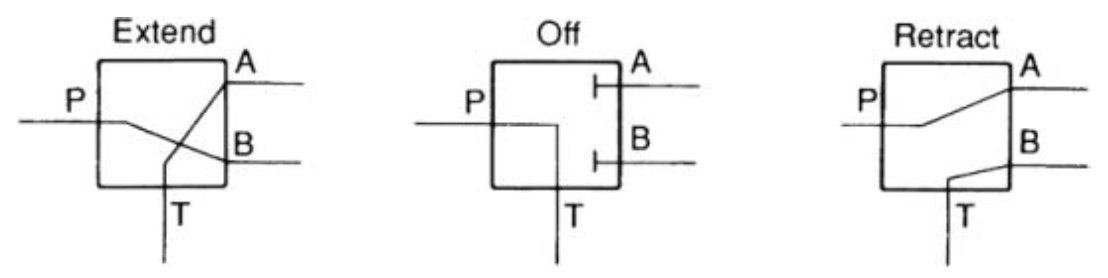
\includegraphics[width = 1\textwidth]{2_images/controlValveConfig.png}
        \caption{4/3 control valve switching configuration~\cite{parr2011hydraulics}.}
        \label{fig:controlValveConfig}
    \end{minipage}\hfill            
    \end{figure}      
    

    All actuators on the lolly machine are driven by 5/2 control valves, this means that each valve has two positions and 5 ports. Figure \ref{fig:5_2Valve} shows a 5/2 pneumatic valve symbol. Valve positions are shown by two square boxes (coloured red and green to clearly illustrate the different positions) each containing two arrows and a T. The arrows show the air flow direction between ports while the T represents a plug. The zigzag on the right hand side of the symbol illustrates a spring, indicating the the control valve is spring return. The rectangle with the diagonal line through the middle shows that a solenoid drives the control action. Figure \ref{fig:cylinderAB} shows the two possible positions of the cylinder.

    \begin{figure}[H]
    \centering
    \begin{minipage}{0.45\textwidth}
        \centering
        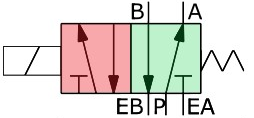
\includegraphics[scale = 0.5]{2_images/5_2Valve.png}
        \caption{A 5/2 pneumatic control valve \cite{5_2Valves}.}
        \label{fig:5_2Valve}
    \end{minipage}\hfill
    \begin{minipage}{0.5\textwidth}
        \centering
        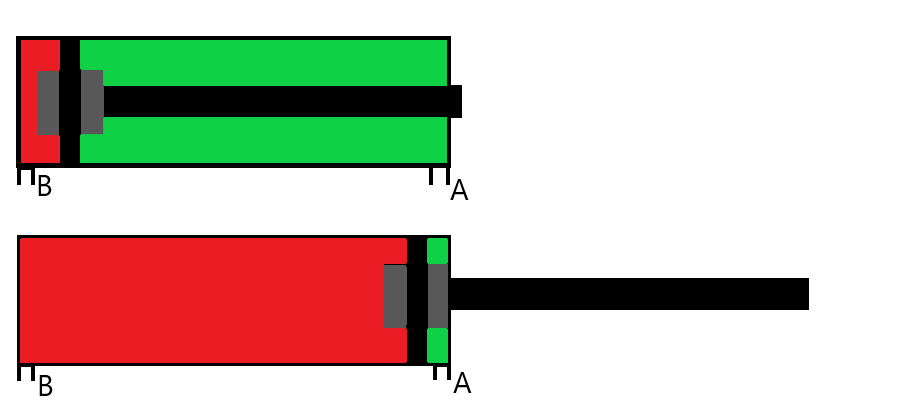
\includegraphics[width = 0.8\textwidth]{2_images/cylinderAB.png}
        \caption{Different cylinder positions. \\Position 1(Top) = Retracted. \\Position 2(Bottom) = Extended}
        \label{fig:cylinderAB}
    \end{minipage}\hfill            
    \end{figure}          
   
   The below position descriptions are in reference to Figure \ref{fig:5_2Valve}.
    \begin{description}
        \item\textbf{Position 1 - Green:}
        While the valve is in position 1 the pressure (P) port is connected to the (A) port and (B) port is connected to the exhaust line (EB).
        \item\textbf{Position 2 - Red:}
        While the valve is in position 2 the pressure (P) port is connected to the (B) side and (A) port is connected the exhaust line (EA). 
    \end{description}
    
 \newpage  
    The control action is what triggers the valve and can vary depending on the application, typical control actions include\cite{parr2011hydraulics}:
    \begin{itemize}
        \item Push Button
        \item Spring
        \item Lever
        \item Roller Limit Switch
        \item Pressure Line
        \item Solenoid
    \end{itemize}
    
    All control valves on the lolly machine are are triggered via solenoid driven pilot valves.